\chapter{The Data Used in This Work}

This chapter presents an overview of the raw data used in this work, the challenges faced when working with higher dimensional data, strategies that were used to overcome these challenges and notes on data re-sampling and spectra region selection. Furthermore, it presents a recent data set of emission-line stars that aided the development of the methods presented in subsequent chapters of this work.

\section{Data Acquisition}

This work utilises the most recent open access spectral data from the GALAH survey. At the time of writing, the GALAH survey is in its third data release (GALAH DR3). GALAH DR3 (hereafter DR3) comprises of 678,423 spectra for 588,571 stars, of which approximately 80\% are within a radius of 2 kpc \citep{buder2021galah+}. DR3 provides continuum normalised spectra and errors for a majority of candidates. Of the 588,571 stars, continuum normalised spectra of 588,343 have been provided. In the case of problematic reductions, for spectra where this is not possible, object IDs and flags have been provided. This study avoids using these problematic spectra.

The data is organised as individual \texttt{.fits} format files. Each file contains an object ID prefix (known as an \texttt{sobject\_id}) followed by the last digit in the filename which serves as a suffix for the camera number. Thus, the file \texttt{1705090057010093.fits} is a data file for an object with \texttt{sobject\_id=170509005701009} and contains spectral data from camera 3 (or the red camera). The blue, green and infrared cameras are denoted by the suffix 1, 2, and 4 respectively.
The red camera of the HERMES spectrograph is the spectral channel with the range 6478\r{A} - 6737\r{A} \citep{sheinis2014first}. This range is of particular interest to this work as the characteristic H$\upalpha$ line appears within this range. These individual files totalling 385 GB were downloaded to a Macquarie University file server and served as the data source for all work presented in this thesis.

\begin{figure}[!htb]
\centering
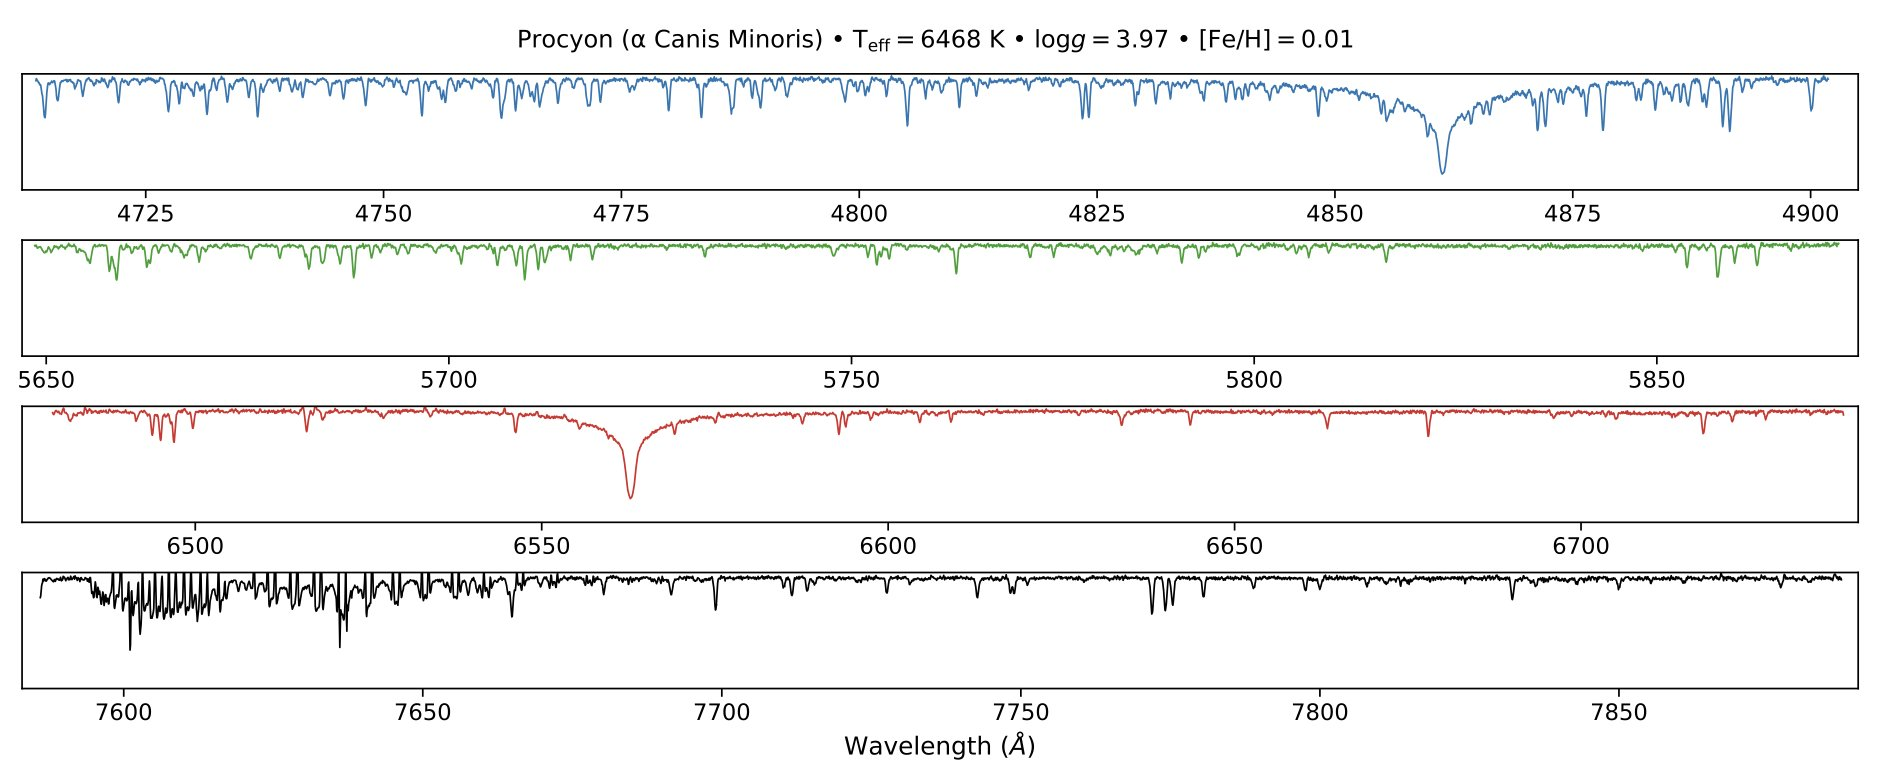
\includegraphics[scale=.25]{figures/galah cameras.jpeg}
\caption{All camera, normalised DR3 spectral data for the star $\upalpha$ Canis Minoris.}
\end{figure}

Feature exploration and engineering is a crucial step when conducting data analysis and in particular for preparation of data prior to the application of machine learning methods. This section provides an analysis of the feature space and search space of DR3 in the context of identifying emission-line stars. The results of this exploratory analysis placed constraints on the design of the machine learning methods discussed in subsequent chapters. Given that spectral features are recorded across four cameras at high resolution, the feature space of DR3 is significant. 

As an illustrative example, consider the red camera only. The feature space calculation is as follows,
\[\lambda_{min} = 6478\]
\[\lambda_{max} = 6737\]
\[\Delta\lambda \approx 0.06\]
$\Delta\lambda$ is the wavelength separation equivalent of the sampling rate of the wavelength grid. Thus the size of the wavelength grid is given by, \[N_{\lambda} = (\lambda_{max}-\lambda_{min})/\Delta\lambda \approx (6737-6478)/0.06 \approx 4317\]
This is the number of features in the red camera for a given spectrum, \[N_{f} \approx 4317\]
Thus the total number of features for the red camera across all available DR3 data is, \[N_{T} \approx 4317\times678,423 \approx \num[round-precision=2,round-mode=figures,
     scientific-notation=true]{2928752091}\]

This calculation naively implies the existence of a billion scale feature space, and consequently a potential billion dimensional vector space. This indicates that the data analysis and machine learning strategy should be planned and managed carefully. If care is not taken during feature engineering and pre-processing steps, the volume of data and complexity will lend itself to what is colloquially referred to as the "curse of dimensionality", which refers to the extraordinarily rapid growth in the difficulty of problems as the number of variables (or the dimension) increases \citep{kuo2005lifting}.

\begin{figure}[!htb]
\centering
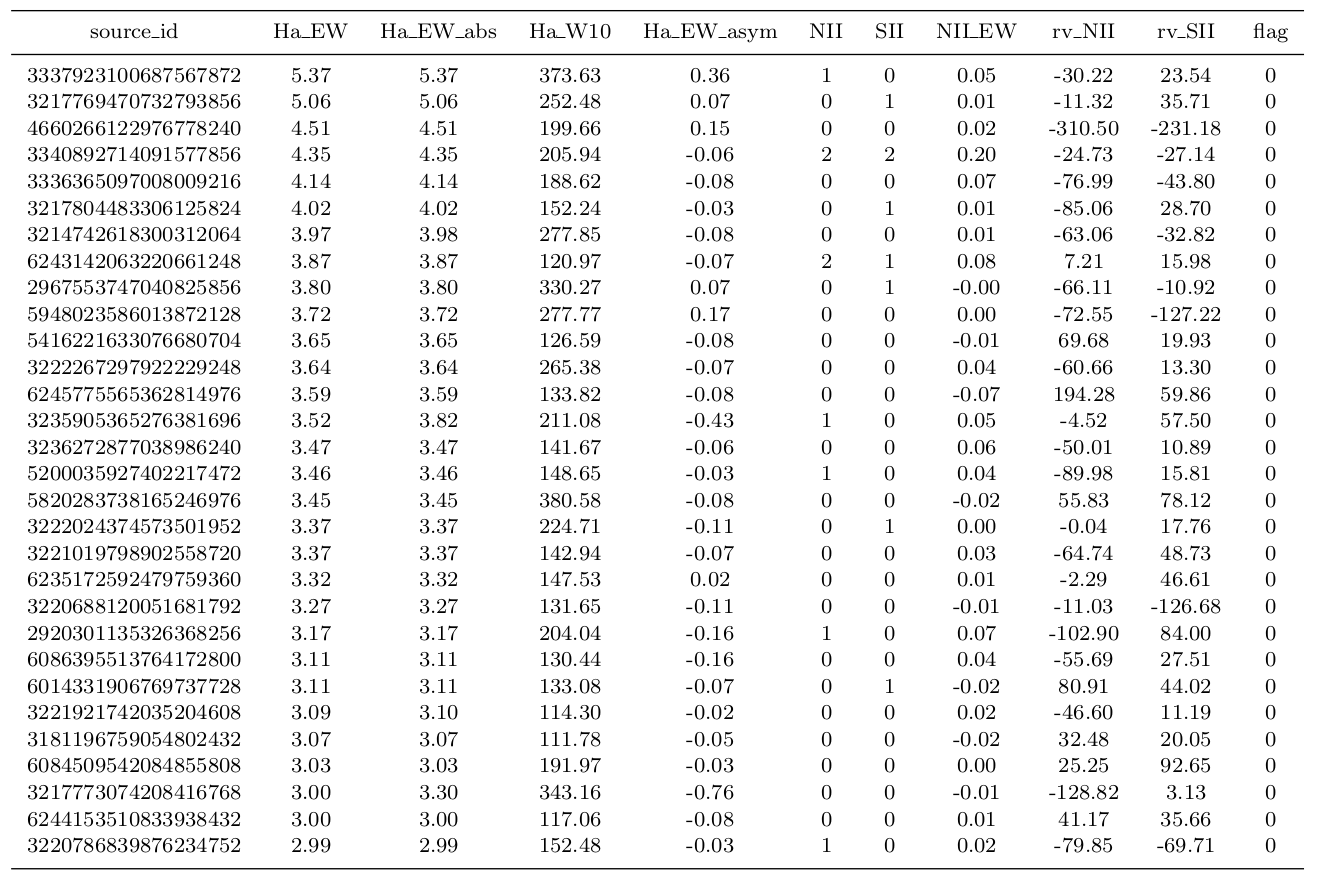
\includegraphics[scale=.45]{figures/cotartable.png}
\caption{The 30 strongest emitters. Reproduced from Čotar et al. \citep{vcotar2021galah}.}
\end{figure}

This work will also utilise a recently published data set of H$\upalpha$ emission line spectra. Published in 2020, Čotar et al. \citep{vcotar2021galah} used a prior version of the GALAH survey \citep{de2015galah}, the K2-HERMES survey \citep{wittenmyer2018k2} and the TESS-HERMES survey \citep{sharma2018tess} to derive a catalogue of potential H$\upalpha$ emission-line spectra using a specific type of neural network known as an autoencoder. Combining data from three surveys, this study used 669,845 continuum normalised stellar spectra as a data input source and included a small fraction of repeated observations. 

The study identified 10,364 emission-line spectra with varying degree of H$\upalpha$ emission components and sub components. Summarised information of these spectra, their object IDs, including GALAH DR3 \texttt{sobject\_ids} were released via \href{https://cdsweb.u-strasbg.fr/}{CDS} as open access data. This summarised data, excluding the continuum normalised spectra, was presented as a single \texttt{.fits} format file. In Chapter 4, this work will demonstrate that a novel clustering approach can identify P Cygni and inverse P Cygni spectra and other species from this sample. Furthermore, this data set was used to benchmark a well established dimensionality reduction based clustering method called t-SNE. These results are presented in Chapter 5. Given the significantly smaller feature and search space, exploring and prototyping methods on this data set proved extremely beneficial when developing the full machine learning method presented in Chapter 6.

\section{Interpreting Spectra as Time Series}

This work takes a unique view of continuum normalised spectra from DR3, casting and interpreting these as one would do a set of time series data points. This proved extremely useful as a mental model when developing the methods presented in this work. This section provides some insights into the motivation for using this mental model. 

A plot of flux recorded by each camera, when presented as a function of wavelength, can be treated mathematically as traditional time series data. While a monotonically increasing time axis is not included in the DR3 data, the monotonically increasing wavelength grid can serve as an analogue to the time axis. Morphologically, the variation of normalised flux against a wavelength grid is analogous to a variable plotted against a time grid \citep{nielsen2019practical}.

This work takes inspiration from this approach. This is an unconventional yet incredibly powerful approach to analysing stellar spectra. Precedent for this approach can be found in related fields such as chemistry and nuclear magnetic resonance (NMR) spectroscopy where NMR spectra are subjected to signal processing methods originally developed for time series analysis \citep{nielsen2019practical}. Viewing spectral data in this manner allowed for the exploration of signal processing methods that are typically reserved for and employed on time series data. Notably, the use of dynamic time warping based clustering was inspired by these mental models. These results are presented in detail in Chapter 4 and 6.

\section{Data Re-sampling}

The DR3 data does not have a constant sampling rate. This implies that the spectra will not have a common wavelength grid and thus makes direct comparison of the morphologies of two spectra challenging. While this rate can be equivalent to $\Delta\lambda$ $\approx$ 0.06 \r{A} \citep{vcotar2021galah} it can vary around this value, particularly in the third decimal place. Furthermore, flux values may not be recorded for all spectra close to $\lambda_{min}$ = 6478 and $\lambda_{max}$ = 6737. Thus when comparing spectra to each other and in particular their morphological features, it was evident that all continuum normalised spectra would have to be re-sampled to a common basis and thus a common wavelength grid. The advantage of this approach is that spectral features, particularly morphological features can be compared against each other more effectively. This work performed this process on data from the red camera only. 

In order to isolate the red camera (camera 3) data, the following file operations were carried out. All filenames of the DR3 \texttt{.fits} format files were read into an array. Files with the suffix "3" were selected. Additionally the number "3" was stripped from this sub array of file names to generate a list of \texttt{sobject\_id} values. This significantly simplifies data querying and reading operations as all standard query and file read operations rely on only \texttt{sobject\_id} and not the combined file name that includes the \texttt{sobject\_id} and camera suffix. The added advantage of this approach is that it automatically excludes \texttt{sobject\_id} values for which red camera data does not exist. A list of such \texttt{sobject\_id} values is published on the GALAH survey website. However this study did not require the use of this list as the procedure above infers these \texttt{sobject\_id} values directly from the \texttt{.fits} filenames. This process results in a collection of 588,344 \texttt{sobject\_id} values. This is lower than the 588,571 total number of stars recorded by DR3. The difference is attributed to those stars for which the normalised red camera data do not exist. 

\begin{figure}[!htb]
\centering
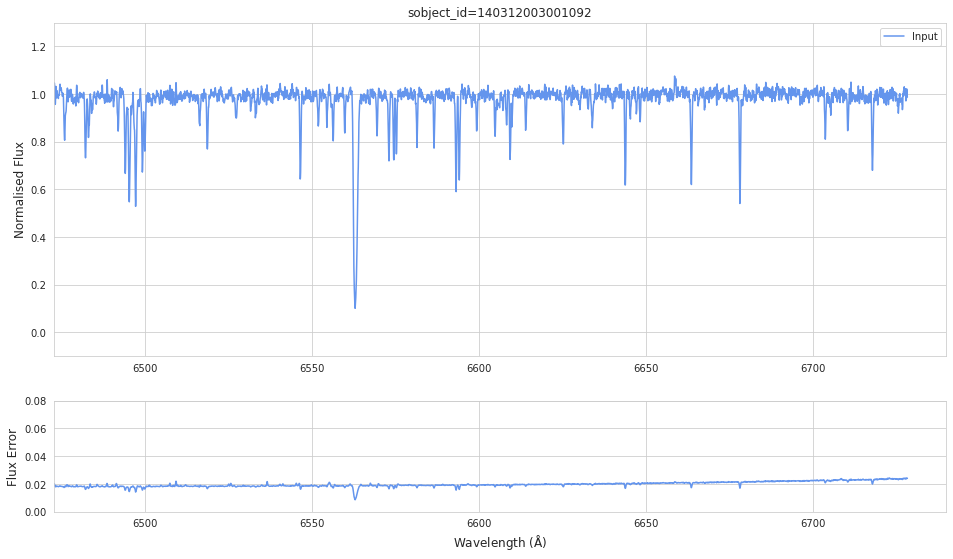
\includegraphics[scale=.40]{figures/input spectrum.png}
\caption{Red camera normalised flux data and error for the \texttt{sobject\_id = 140312003001092}, prior to re-sampling.}
\end{figure}

To significantly minimise over-sampling and under-sampling, the spectra under consideration were interpolated to a common wavelength grid with a sampling rate equivalent to 0.06 \r{A}. This rate is accurate to the sampling rate of each spectrum generated by the red camera to the second decimal place.

\begin{figure}[!htb]
\centering
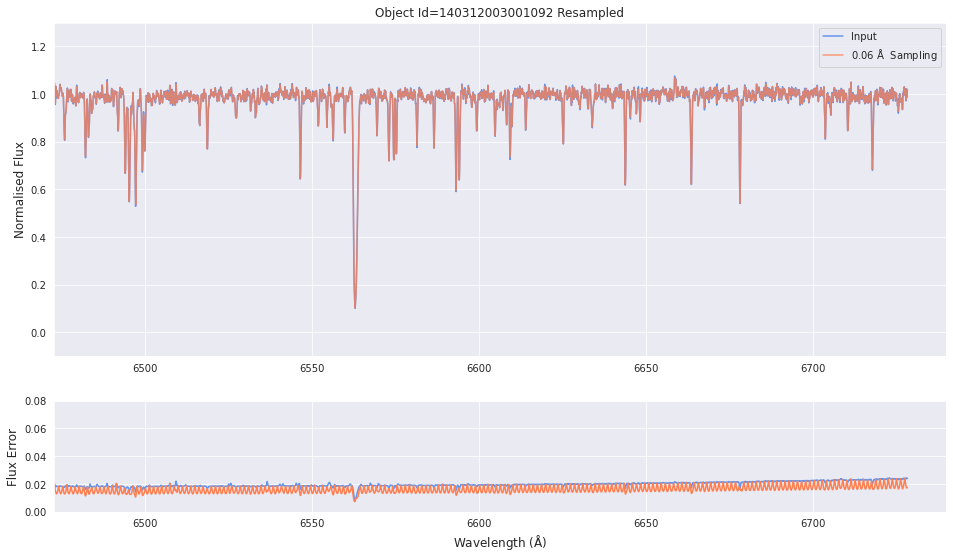
\includegraphics[scale=.40]{figures/resampling example.png}
\caption{\texttt{sobject\_id = 140312003001092}, re-sampled.}
\end{figure}

This work used the \texttt{spectres} Python package \citep{carnall2017spectres} to efficiently sample all red camera spectra to the following common wavelength grid.

\[\lambda_{min} = 6472.5\]
\[\lambda_{max} = 6740\]
\[\Delta\lambda = 0.06\]

This grid was chosen based on the range of wavelength separation observed in the raw data as well as the work of Čotar et al. Normalised spectra and their errors from the red camera were subjected to this process. The authors of DR3 have set the continuum value for the normalised spectra at 1. Thus, spectra for which flux values were not recorded at the tail and top end of the interpolated grid, were padded with the value 1 in order to maintain the uniformity of the common wavelength grid. Re-sampling is computationally intensive and thus this process was offloaded to a university server. The resultant data and interpolated errors were saved as HDF5 files using the \texttt{.h5} file format in a single array for convenience. 

\section{Region Selection}

This work exploited the use of effective spectral region selection to reduce the feature and search space as well the memory and disk footprint. It was demonstrated previously that the total number of spectral features for the red camera is $\sim$ \num[round-precision=2,round-mode=figures, scientific-notation=true]{2928752091}. P Cygni, inverse P Cygni and other emission-line stars considered in this work show characteristic emission and absorption profiles near the H$\upalpha$ line. This observation can be used to significantly reduce the size of the feature space. 

The region of interest around H$\upalpha$ was selected to be 6561\r{A} - 6565\r{A} \citep{traven2017galah}. By repeating the feature space calculation above it can be noted that this region is sufficiently narrow enough to reduce the feature space by a hundredfold to $\sim$ \num[round-precision=2,round-mode=figures, scientific-notation=true]{45228200} while simultaneously ensuring that it can encapsulate the emission features under consideration. 

In code, this selection was implemented as a binary spectral mask which extracts the flux values for the relevant wavelength range while masking flux values outside this range. A masked version of the re-sampled data was stored in a separate \texttt{.h5} file for convenience. In terms of memory and disk allocation, this had the effect of reducing the memory footprint from $\sim$60GB for the re-sampled red camera data to $\sim$1GB for the H$\upalpha$ masked version of the same data. This improved the speed of read/write operations significantly. 

\section{Concluding Remarks}

This work draws the following conclusions from the analysis presented above,

\begin{enumerate}
\item When faced with higher dimensional data, dimensionality reduction and sample size pruning can be effective strategies when seeking to identify and classify atypical emission-line spectra. 

\item Open data sets such as that provided by Čotar et al. can be useful as a prototyping aid to iteratively develop and evaluate machine learning methods given the low volume of data compared to GALAH DR3. 

\item Re-sampling can ensure that all spectra can be compared on the same wavelength grid. This is particularly useful for developing machine learning methods as the consistency of the data can be maintained throughout the process, particularly when comparing morphologies of spectra.  

\item Region selection can significantly reduce the feature space and search space by efficiently limiting it to those only the regions that are of interest for a particular study. 
\end{enumerate}

